\section{Results and Discussion} \label{results}



\subsection{Performance}\label{performance}
The temporal dynamics of a molecular system can be described by the \acrfull{cme}\citationneeded{CME reference}.
\acrfull{gssa}\cite{gillespie_general_1976} simulates these stochastic dynamics directly returning a set of individual trajectories for a list of particles observed.
In order to obtain accurate estimates of the average dynamic within a population of cell (\ie{} the mean dynamics), it is however necessary to perform multiple (often more than $10^4$) simulations.
Despite recent efforts \cite{niemi_efficient_2011,dittamo_optimized_2009,komarov_accelerating_2012} to provide fast implementation of this algorithm, computation remains extremely expensive. 
This time-complexity is a limiting factor in downstream analysis techniques, for
instance parameter inference that often requires repetition of these experiments for a large set of parameter values.

This particular limitation led to the development of approximations such as \acrfull{lna}\cite{komorowski_bayesian_2009} and \acrfull{mea}\cite{ale_general_2013}
 which model the mean behaviour directly, without evaluating the individual particle behaviours, and therefore can perform in a more realistic time.

Since the main driving force for development of these approximation algorithms is the potential reduction of the time taken to perform the analysis, 
it is paramount to make the implementation as efficient as possible.

In this section, we explore the implementation factors that influence the runtime of the algorithm, and describe the optimisations done to increase the its performance.
In particular, we show that symbolic computations can be limiting the algorithm and explain the techniques used to optimised them.
We also quantify the increase in performance we achieved and show that it is several orders of magnitude faster than the original \mat{} implementation.
In addition, we explore other limiting factors we have less control of, such as the choice of \gls{ode} solver, and discuss their potential implications to the analysis of biological systems.

\subsubsection{Optimising \acrlong{mea}}
\label{sec:optimising_mea}

\gls{mea} involves derivation of a system \gls{ode}s from a model.
This procedure\cite{ale_general_2013}, involves lengthy symbolic calculations.
Even for very simple models (\eg{} three species, five reactions), they cannot be realised manually.
The number equations in the generated \gls{ode} system, for a model with $s$ species and up to moments of order $o$ can be estimated by the following equation: 
\begin{displaymath}
    \text{Number of equations} = {{s + o} \choose {s}} - 1
\end{displaymath}
As a consequence, the complexity of the calculation is predicted to increase exponentially with the number of species in the system and the maximal order of moments. 
For example, in a system with five species,  performing \gls{mea} up to moments of order 2, 3, 4 and 5, results in an \gls{ode} system with  20, 55, 125 and 251 equations, respectively. 

%In order to perform symbolic computations, we have used \sympy{} \cite{sympy_development_team_sympy:_2014}; a \py{} implementation of
%the symbolic computation routines.

In order to increase the scalability of the method, we have identified significant bottlenecks in our procedures using \py{} profiling tools.
We have then attempted to iteratively remove these bottlenecks one by one. Figure~\ref{fig:mea_speed} shows the cumulative effects of different optimisations.
The performance assessment were realised on algorithm when performing log-normal closure in order to show the effect of improvements specific to parametric closure (fig.~\ref{fig:mea_speed}d). 

\begin{figure}[tbh]

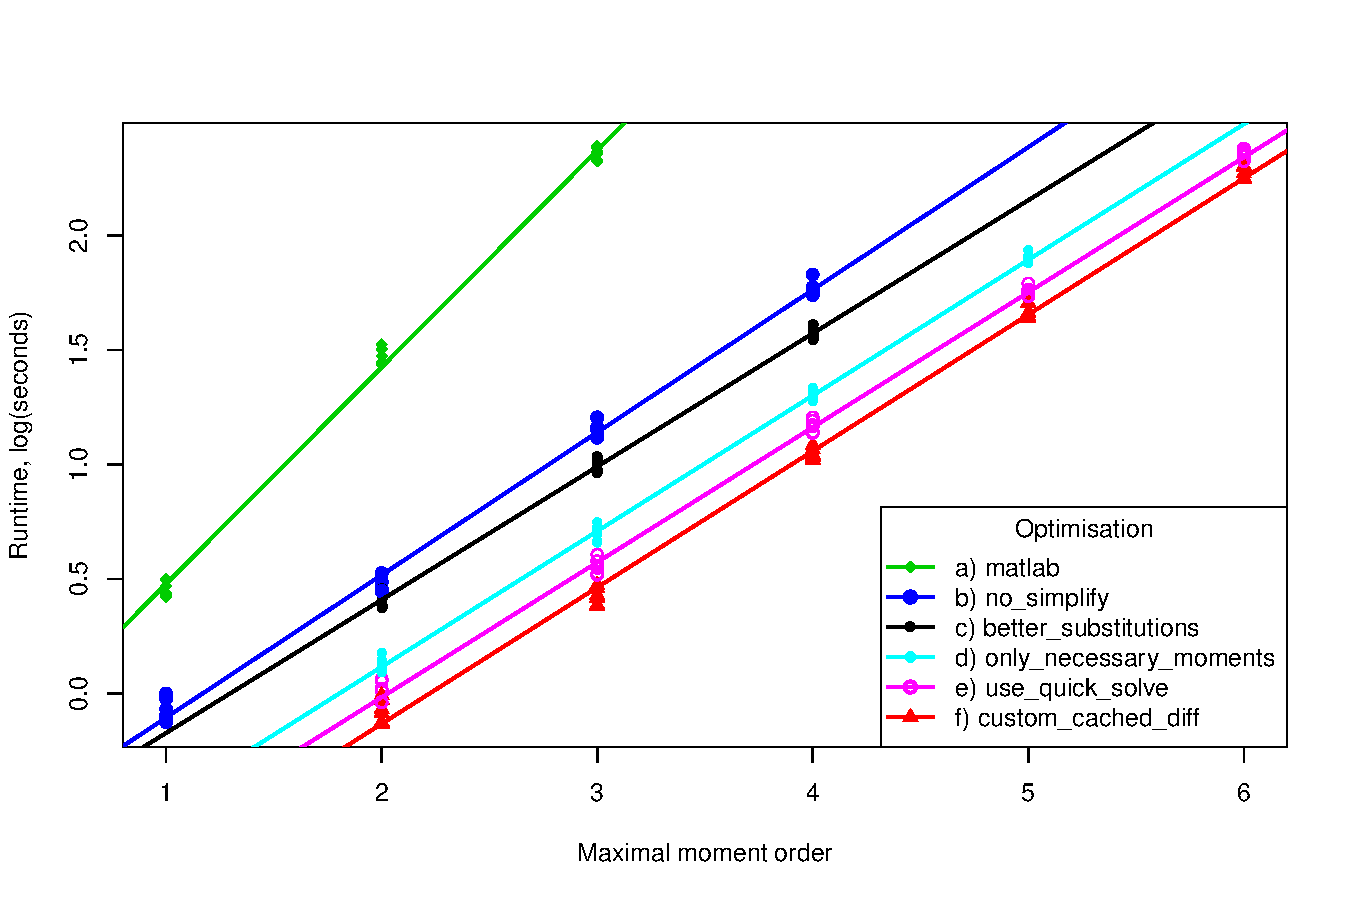
\includegraphics[width=1.0\textwidth{}]{../figure_mea_speed/mea_speed.pdf}
\caption{\emph{Cumulative performance improvement of symbolic calculations resulting from optimisation}.
The processing time for computing log-normal closure on \pft{} model with different maximal moment orders were measured for original Matlab implementation (a) and different optimisations (b$-$f).
In a first place, the calls to \texttt{sympy.simplify()} where removed (b). 
Then, \texttt{sympy.xreplace()} was used instead of \texttt{sympy.substitute()} (c). 
Generating an $(n-s) \times (n_2-s + 1)$ matrix (d), as opposed to an $(n-s) \times (n-s + 1)$ one, also increase speed.
Implementing a simplified equation solver instead of using \texttt{sympy.solve()} also resulted in a significant speed-up (e). Finally, caching (memorisation) \texttt{sympy.diff()} allowed even better performance.
The time complexity appears exponential ($O(2^n)$, where $n$ is the maximal moments order) in every case, 
Interestingly, the slopes between, a ($0.95$) and c ($0.58$), and b ($0.62$) and c were significantly different ($p-value <10^{-15}$ and $p-value = 3 \times 10^{-4}$, respectively; t-test on the slopes of the linear regression). 
No significant difference was found between the slopes of the subsequent optimisations (c$-$f). 
However, the intercepts were significantly smaller between each consecutive optimisations after c) ($p-value < 10^{-6}$ for all; t-test on the intercepts of the linear regression).
Nine replicates were performed on the same CPU. For optimisation c$-$f, values corresponding to maximal order moments lower than two were removed because of the inherent inaccuracy in measuring very short durations}
\label{fig:mea_speed}
\end{figure}



Reorganising, profiling and rewriting the code resulted in incremental significant performance improvements of symbolic computations in \means{} compared to the original \mat{} code.
For instance, with the same \pft{} system and closure method, 
we predict that computation up to \gls{ode}s up $8^{th}$ order will take 46 minutes with \means{}, 5 hours after the first optimisation (fig.~\ref{fig:mea_speed}b) and as much as 148 days with the original implementation.
These improvement have allowed us to explore the performance of MEA in higher depth, and will hopefully contribute to make \gls{mea} realistically usable for systems with more species and reactions.

\subsubsection{Evaluating Trajectories Efficiently}

\todo[inline]{New Section: Somebody please review}

As mentioned in the introduction to this section, the reduction of computational cost was the key driving factor for development of approximation methods.
As described in the previous section, in order to be able to explore the approximation methods in more depth, we need to make the generation of the set of equations as efficient as possible. 

Even though it is a great improvement from the original prototype, 46 minutes is still a long time to wait for the computer to do the number crunching. We can accept to wait this long, however, as we only need to do that once for a set of equations -- the next time we intend to do that, we can just read the previous set from a file.

Evaluating these expressions is a completely different story however.
Since we need to evaluate each expression hundreds, if not thousands of times when performing the simulations of the system, we want to make these tasks as efficient as possible, as every microsecond counts. 

In order to minimise the overhead of computations, we use the {\tt autowrap} module, built into {\tt sympy} to compile our numeric expressions into C and wrap the python interface around them so the end user does not see any difference. This process adds some overhead when the first evaluation is performed, as the system needs to be compiled, however the subsequent evaluations are orders of magnitude faster (illustrated in the \autoref{sec:reuse_of_simulation_objects}).


\subsection{Moment Expansion Closure}

In \gls{mea} the time derivative of each central moment is expressed in terms of the higher order moment. 
This behaviour essentially has no upper bound and continues to the moments of infinite order. 
Since we cannot evaluate these expressions in the limit analytically, it is necessary to ``close'' the expansion by providing a closed form for the higher order moments.
This also makes the method an ``approximation" rather than an exact method.

In the original work \cite{ale_general_2013}, higher order central moments are assumed to be equal to zero.
This is very convenient, but is a strong and not necessarily valid assumption. 

As an alternative, parametric probability distribution can be used to express moments of arbitrary orders. 
For instance, a multivariate normal distribution is parametrised only by means (\ie{} first order raw moment)
and a covariance matrix (\ie{} second order central moments). 
As a consequence, it is possible to express any arbitrary moment from means, variances and covariances. 
A promising area of research involves closing moment expression by parametric forms of highest order central moments instead
of assuming them to be null.
Preliminary work \citationneeded{Eszter, unpublished} suggests that using a parametric distributions for \gls{mea} is, in some cases, a better approximation.
In addition, Ale \emph{et al.} predicted that ``including more moments would improve the estimation''\cite{ale_general_2013}.

The dramatic improvement in performance compared to the \mat{} prototype (see \autoref{sec:optimising_mea}) has rendered the exploration of higher-order and parametric moment closures possible.
Therefore, we were naturaly interested in investigating the effect of maximal moment order and different type of closures on the quality of the approximation.
igure~\ref{fig:max_order_and_closure_on_distance_summary} summarises our resutlts on the \pft{} model.

\begin{figure}[t]
    \centering
    \includegraphics[width=1.0\textwidth]{../pipeline/task-output/FigureP53Summary/FigureP53Summary-pdf-7.pdf}
    \caption{\emph{Effect of different closure methods and maximal moment order on simulation accuracy}. The \pft system was modelled using \gls{mea} with five types of closure and for maximal moment order up to seven.
Resulting trajectories were all compared to an average of 5000 \gls{gssa} simulations using sum of square distance (a).
Distance is in log scale. Missing values indicate solver failure for that particular set of parameters.}
    \label{fig:max_order_and_closure_on_distance_summary}
\end{figure}

The \pft{} system, with parameters from \cite{ale_general_2013}, was investigated.
As mentioned earlier it is expected that the approximation accuracy increases with the maximal moment order, \ie{} distance to \gls{gssa} obtained should decreases
 as maximal moment order increases. 
For normal and scalar closures, this trend we observe this trend up to maximal moment order six. 
However, this does not stand for seventh order moment.

\quentintodo[inline]{Todo double check the labels in the legend, was it really normal that was worse and scalar that failed?}

As seen in the figure, the closure using the normal distribution had performed worse than the sixth order closure when maximum order was set to seven.
We could not obtain the result for the seventh order closure using the standard scalar closure, as the ODE solver has failed simulating the problem, which usually indicates a ``stiff'' \gls{ode} problem\citationneeded{stiff odes}. 
The generated trajectories are shown in \autoref{fig:max_order_and_closure_on_distance_trajectories}. 
Trajectory generated from the normal distribution closure seem to `mismatch' the trajectory obtained from the \gls{gssa} simulations by a margin.
% (\emph{purple line, subplot on the right-hand-side}). 

The reason for this behaviour is uncertain; it might be a limitation of the approximation method, or a numerical limitation of the available \gls{ode} solver.
It is hard to know which explanation is more likely since we cannot test the two hypotheses separately. 
Interestingly, we observed a similar behaviour with all of the solvers tested, which is further explored in \sauliustodo{link to my section where we study the phenomenon on larger scale with different solvers}.

Note that for even maximal moment orders, normal and scalar are identical.
When the maximal moment order is even, it means that the perametric expression of an odd (the next) order moment was used for closure.
Normal distribution is symmetrical. One consequence is that odd central moments are always zero. 
For instance, the sckew (\ie{} third order central moment) of a normal distribution is zero.
Therefore, this behaviour is perfecty normal.


\begin{figure}
    \centering
    \includegraphics[width=1.0\textwidth]{../pipeline/task-output/FigureP53Simple/FigureP53Simple-pdf-7.pdf}
    \caption{\emph{Complete trajectories of a single species (\pft) for max order three and seven are shown} Black lines indicate the average of \gls{gssa} simulations. 
    Missing lines, compared to the legend in \autoref{fig:max_order_and_closure_on_distance_summary} indicate solver failure.}
    \label{fig:max_order_and_closure_on_distance_trajectories}
\end{figure}

 
for log-normal closure, the ground truth trajectory seems to be well approximated when the maximal moment order is three, but the approximation gets less and less accurate for higher maximal order moments.
A deeper look at the trajectories indicate that, in this latter case,
oscillations are damped too quickly, as opposed to the behaviour seen using normal closure, where the oscillation amplitude increases (see \autoref{fig:max_order_and_closure_on_distance_trajectories}, red line).

Interestingly, for even maximum moment order (\ie{} 2, 4, 6) log-normal closures generated \gls{ode}s which, despite our efforts, could not be numerically solved.

Finally, it seems that the results obtained from multivariate distribution closures and  univariate distribution closures, which do not model the covariance terms, are the same for this particular system. 
This is not true for all of the systems. 
For instance, we have observed that in the \emph{hes1}, it is advantageous to model covariance (data not show).
\quentintodo{put hes1 exple if time}

Surprisingly, higher order moment closure did not necessarily result in better approximations.
In addition, our results indicate that there might be a complex interaction between the type of closure and the maximal moment order. 
Unfortunately, this makes it difficult to define \emph{a priori} which closure and maximal moment order should be used for a given system.
These unexpected results lead us explores this phenomenon on wider scale of parameters\sauliustodo{link to the section}.

\subsection{Parameter Inference using \acrlong{mea}}
Parameter inference procedure aims to obtain the correct parameter values for the system by exploring the parameter space and comparing the simulation trajectories with the experimental data. 

In order to study the performance of the parameter inference procedure using \acrlong{mea}, we took the average trajectory obtained from the  $5000$ \gls{gssa} simulations of the \pft{} with a certain parameter set and used it as the observed dataset we want to infer the parameters from. Essentially, the inference procedure is expected to return the said parameter set back to us.

In order to determine the base case performance, we performed the parameter inference using the \pft{} model expressed only in terms of the first order moments. This approximation is bound to be very inaccurate for the particular system, as higher order moments are necessary to capture the damped oscillations present in the means of \gls{gssa} simulations\cite{ale_general_2013}\sisitodo{figure is needed}.

We have decided started parameter inference procedure at the correct parameter values, expecting to see an immediate result and no movement in the parameter space. To much of our surprise, however, when the inference is allowed to navigate the complete parameter space, not only did the procedure the procedure did move around, but it was able to find a set of parameters, that when expressed in terms of first order moments, are able to match the observed trajectories completely.

The set of parameters obtained by the inference were very different from the actual SSA simulations, but the approximated trajectories were identical. This strongly questions the suitability of parameter inference procedures in obtaining the correct parameter sets.

\sisitodo[inline]{Need figure here showing that they are really close}
\sisitodo[inline]{Why don't we compare the SSA trajectories with these parameters somewhere as well, if there is time?}

In order to gain some insight into what is happening, we first attempted to restrict ourselves to easier to comprehend two-dimensional space.
To do this, we restricted our parameter inference procedure to only move through pair of parameters only, while all other parameters are fixed (to their true values). 
We performed this for all combinations of two parameters and checked if we can reproduce the curious behaviour.

Interestingly, we were able to observe the same behaviour for the parameter pairs ....
\sisitodo[inline]{list the parameter pairs that work, add figure for $c_2$, $c_6$.}
We have chosen the pair of parameters that allowed the inference procedure to converge to a trajectory with minimal distance to the stochastic average -- $c_2$ and $c_6$ for further investigations.

\sisitodo[inline]{look up autoref function, and refer to correct figure, it is not Figure 5 any more, as it was before}
 
\sisitodo[inline]{See the commented text below this todo -- instead of it please talk a bit more about how the landscape looks for the max\_order = 1. Then go on and talk about higher-order moments, explicitly mentioning that you were able to find close-enough trajectories for all of them, however, neither of them were accurate parameter wise}
%If the inference method was correct, the starting point in the distance landscape would already have a low distance, and the end point should overlap with the starting point, i.e. the true values of $c_2$ and $c_6$.

In conclusion, the data makes us question the validity of parameter inference approaches using \gls{mea} approximation.
As seen in \sisitodo{remind which figures} distance landscape shows that the starting point (which is the correct parameter set) can be distant from the minima. Similarly, the distance procedure, if uncontrolled, is able to find itself exploring the values for some parameters (i.e. $c_6$) that are more than 10 times larger than the true value, which not be very meaningful biologically.\sisitodo{great point, but also needs coverage above}
\sisitodo{not clear what you meant here}Finally, the trajectories for all the species in the p53 model sometime demonstrate misfit between the optimal trajectory obtained from inference and the "observed trajectory" from \gls{gssa}. 

\sisitodo[inline]{I think you should structure your figures as you did initially -> the landscape on the left, trajectories on the right, and have one figure per combination of the two}

\begin{figure}
\centering
    \begin{subfigure}[t]{0.2\textwidth}
    \includegraphics[width=\textwidth]{{../pipeline/task-output/SampleMultidimensionInferenceFigure/SampleMultidimensionInferenceFigure-pdf-1-scalar-True-90.0_0.002_1.704_1.1_0.93_0.96_0.7822-ode15s--90.0_0.002_1.704_1.1_0.93_0.96_0.7822-sum_of_squares-5000}.pdf}
    \end{subfigure}
    \begin{subfigure}[t]{0.2\textwidth}
    \includegraphics[width=\textwidth]{{../pipeline/task-output/SampleMultidimensionInferenceFigure/SampleMultidimensionInferenceFigure-pdf-2-scalar-True-90.0_0.002_1.704_1.1_0.93_0.96_0.7822-ode15s--90.0_0.002_1.704_1.1_0.93_0.96_0.7822-sum_of_squares-5000}.pdf}
    \end{subfigure}
    \begin{subfigure}[b]{0.2\textwidth}
    \includegraphics[width=\textwidth]{{../pipeline/task-output/SampleMultidimensionInferenceFigure/SampleMultidimensionInferenceFigure-pdf-3-scalar-True-90.0_0.002_1.704_1.1_0.93_0.96_0.7822-ode15s--90.0_0.002_1.704_1.1_0.93_0.96_0.7822-sum_of_squares-5000}.pdf}
    \end{subfigure}
    \begin{subfigure}[b]{0.2\textwidth}
    \includegraphics[width=\textwidth]{{../pipeline/task-output/SampleMultidimensionInferenceFigure/SampleMultidimensionInferenceFigure-pdf-4-scalar-True-90.0_0.002_1.704_1.1_0.93_0.96_0.7822-ode15s--90.0_0.002_1.704_1.1_0.93_0.96_0.7822-sum_of_squares-5000}.pdf}
    \end{subfigure}
    \begin{subfigure}[b]{0.2\textwidth}
    \includegraphics[width=\textwidth]{{../pipeline/task-output/SampleMultidimensionInferenceFigure/SampleMultidimensionInferenceFigure-pdf-5-scalar-True-90.0_0.002_1.704_1.1_0.93_0.96_0.7822-ode15s--90.0_0.002_1.704_1.1_0.93_0.96_0.7822-sum_of_squares-5000}.pdf}
    \end{subfigure}
    
\caption{\emph{Distance landscape at different maximal orders for p53 model.} In the landscape, the warmer the colour, the more distant the inferred trajectories are from the \gls{gssa} trajectories. 
The \gls{gssa} trajectories are generated using the new parameter values labelled as \emph{start}. Among seven parameters, only the values for $c_2$ and $c_6$ are inferred, with starting values inferred from inference using the true values.} 
\label{fig:parameter_inference_landscape}
\end{figure}

\begin{figure}
\centering
    \begin{subfigure}[b]{0.6\textwidth}
    \includegraphics[width=\textwidth]{{../pipeline/task-output/FigureInferenceStartEndSSA/FigureInferenceStartEndSSA-1-scalar-c2-1.7040-c6-0.7822}.pdf}
    \end{subfigure}
    \begin{subfigure}[b]{0.6\textwidth}
    \includegraphics[width=\textwidth]{{../pipeline/task-output/FigureInferenceStartEndSSA/FigureInferenceStartEndSSA-2-scalar-c2-1.7040-c6-0.7822}.pdf}
    \end{subfigure}
    \begin{subfigure}[b]{0.6\textwidth}
    \includegraphics[width=\textwidth]{{../pipeline/task-output/FigureInferenceStartEndSSA/FigureInferenceStartEndSSA-3-scalar-c2-1.7040-c6-0.7822}.pdf}
    \end{subfigure}
    \begin{subfigure}[b]{0.6\textwidth}
    \includegraphics[width=\textwidth]{{../pipeline/task-output/FigureInferenceStartEndSSA/FigureInferenceStartEndSSA-4-scalar-c2-1.7040-c6-0.7822}.pdf}
    \end{subfigure}
    \begin{subfigure}[b]{0.6\textwidth}
    \includegraphics[width=\textwidth]{{../pipeline/task-output/FigureInferenceStartEndSSA/FigureInferenceStartEndSSA-5-scalar-c2-1.7040-c6-0.7822}.pdf}
    \end{subfigure}
\caption{\emph{Trajectories for each species in p53 model using different maximal orders.} 
Three trajectories are shown for each species. 
The starting trajectories are simulated using the starting values are indicated above the trajectories, with $c_2$ and $c_6$ inferred using \emph{sum of squares} distance method. 
Both the optimal and the \gls{gssa} trajectories are generated based on the end point in correspondent distance landscape in Figure 5.} 
\label{fig:parameter_inference_trajectories}
\end{figure}
